\documentclass{beamer}
\usepackage[orientation=portrait,size=a0,scale=1.4,debug]{beamerposter}
\mode<presentation>{\usetheme{ZH}}
\usepackage{chemformula}
\usepackage[utf8]{inputenc}
\usepackage[german, english]{babel} % required for rendering German special characters
\usepackage{siunitx} %pretty measurement unit rendering
\usepackage{hyperref} %enable hyperlink for urls
\usepackage{ragged2e}
\usepackage{color}
\usepackage{amsmath}
\usepackage{amssymb}
\usepackage{natbib}


\usepackage{array,booktabs,tabularx}
\newcolumntype{Z}{>{\centering\arraybackslash}X} % centered tabularx columns

\title{\huge The Cosmic Abundance of Molecular Hydrogen}
\author{Thomas Fletcher, Supervisor: Dr. Amélie Saintonge}
\institute{Department of Physics and Astronomy, University College London}
\date{June 29, 2016}

\newlength{\columnheight}
\setlength{\columnheight}{105cm}

\begin{document}
\begin{frame}
\begin{columns}
	\begin{column}{.5\textwidth}
		\begin{beamercolorbox}[center,wd=\textwidth]{postercolumn}
			\begin{minipage}[T]{.95\textwidth}  % tweaks the width, makes a new \textwidth
				\parbox[t][\columnheight]{\textwidth}{ % must be some better way to set the the height, width and textwidth simultaneously
%%%%%%%%%%%%%%%%%%%%%%%%%%%%%%%%%%%%%%%%%%%%%%%%%%%%%%%%%%%%%%%%%%%%%%%%%%%%%%%%
					\begin{myblock}{\LARGE Introduction}
						This is the introduction. \cite{keres2003co}
					\end{myblock}\vfill
%%%%%%%%%%%%%%%%%%%%%%%%%%%%%%%%%%%%%%%%%%%%%%%%%%%%%%%%%%%%%%%%%%%%%%%%%%%%%%%%
					\begin{myblock}{\LARGE COLD GASS Results}
						\begin{figure}[H]
						  \centering
						  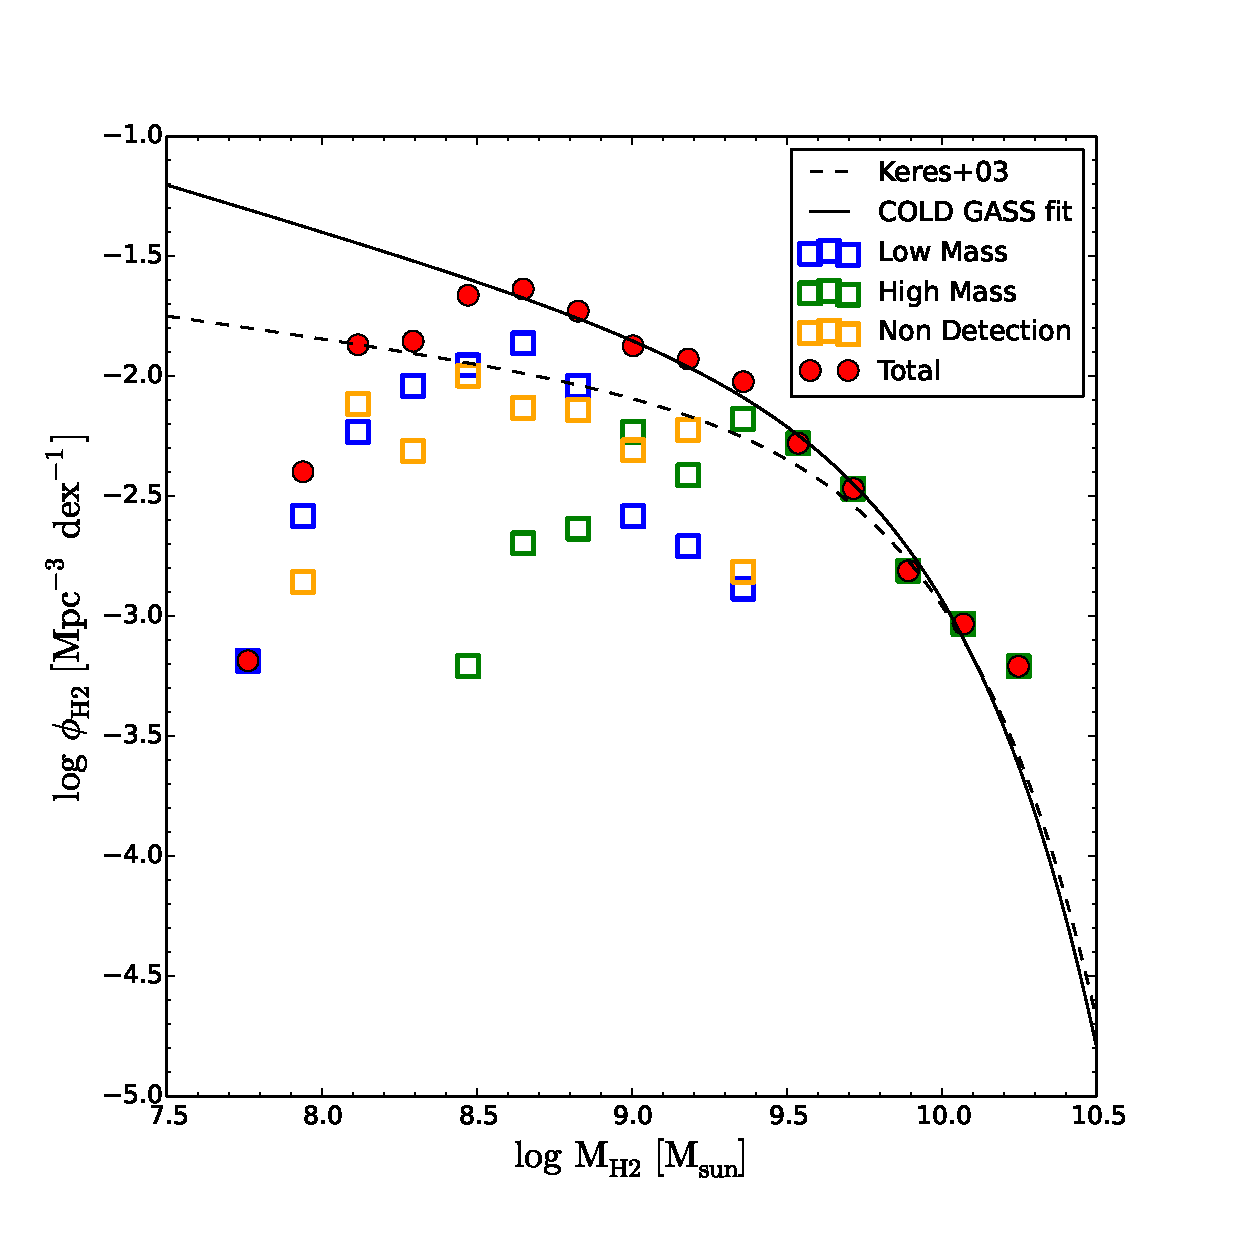
\includegraphics[width=\textwidth]{img/MH2.eps}
						  \caption{Molecular gas mass function ($\mathrm{M_{H2}}$).
							The blue, green and orange squares represent the low mass, high
							mass and non-detections from the COLD GASS survey and the red
							circles how the total contribution from all galaxies in the
							survey. The dashed line is the best fit from \cite{keres2003co}
							and the solid line is the best fit to the COLD GASS data.}
						  \label{fig:2013GasFraction}
						\end{figure}
						\begin{equation}
							\mathrm{\Omega_{H2} = 3.1 \cdot 10^{7} ~ M_{\odot}~ Mpc^{-3}}
						\end{equation}
					\end{myblock}\vfill
%%%%%%%%%%%%%%%%%%%%%%%%%%%%%%%%%%%%%%%%%%%%%%%%%%%%%%%%%%%%%%%%%%%%%%%%%%%%%%%%
\begin{myblock}{\LARGE Conclusions}
\end{myblock}\vfill
%%%%%%%%%%%%%%%%%%%%%%%%%%%%%%%%%%%%%%%%%%%%%%%%%%%%%%%%%%%%%%%%%%%%%%%%%%%%%%%%
		}\end{minipage}\end{beamercolorbox}
	\end{column}
%%%%%%%%%%%%%%%%%%%%%%%%%%%%%%%%%%%%%%%%%%%%%%%%%%%%%%%%%%%%%%%%%%%%%%%%%%%%%%%%
	\begin{column}{.5\textwidth}
		\begin{beamercolorbox}[center,wd=\textwidth]{postercolumn}
			\begin{minipage}[T]{.95\textwidth} % tweaks the width, makes a new \textwidth
				\parbox[t][\columnheight]{\textwidth}{ % must be some better way to set the the height, width and textwidth simultaneously
%%%%%%%%%%%%%%%%%%%%%%%%%%%%%%%%%%%%%%%%%%%%%%%%%%%%%%%%%%%%%%%%%%%%%%%%%%%%%%%%
					\begin{myblock}{\LARGE Methods}

					\end{myblock}\vfill
%%%%%%%%%%%%%%%%%%%%%%%%%%%%%%%%%%%%%%%%%%%%%%%%%%%%%%%%%%%%%%%%%%%%%%%%%%%%%%%%
					\begin{myblock}{\LARGE Scaling Relations}
						The second method makes use of tight scaling relations in the
						$\mathrm{M_{*}-SFR}$ plane
						\begin{figure}
							\begin{minipage}{0.32\textwidth}
								\centering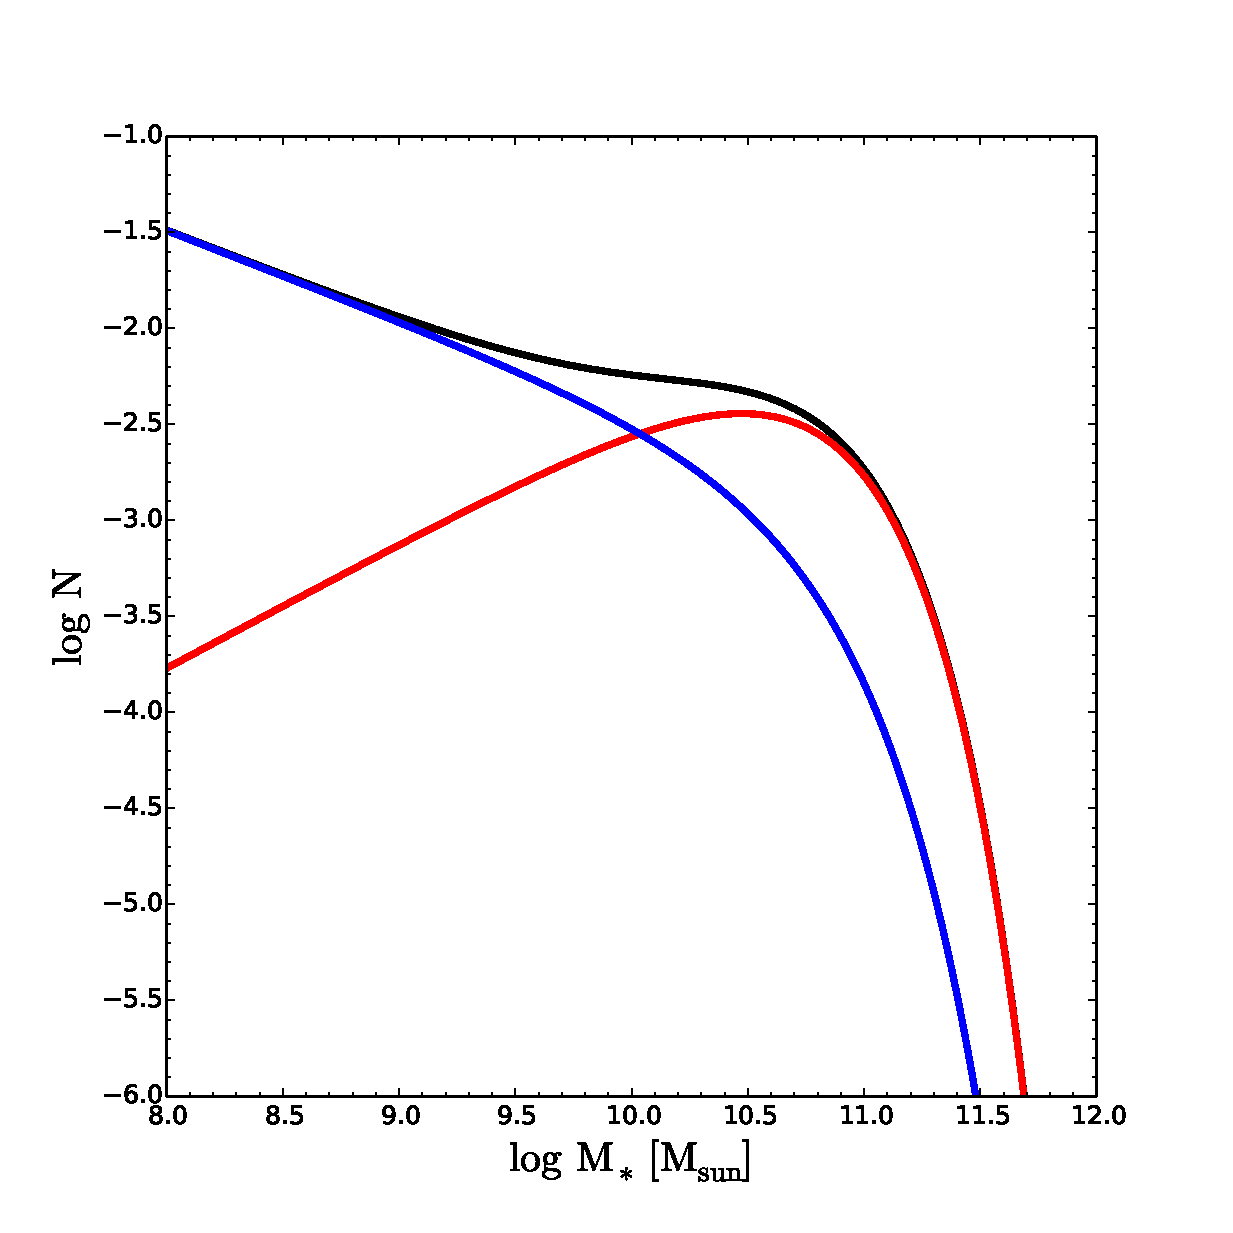
\includegraphics[width=\textwidth]{img/Baldry.eps}
								\caption{}
							\end{minipage}
							\begin{minipage}{0.32\textwidth}
								\centering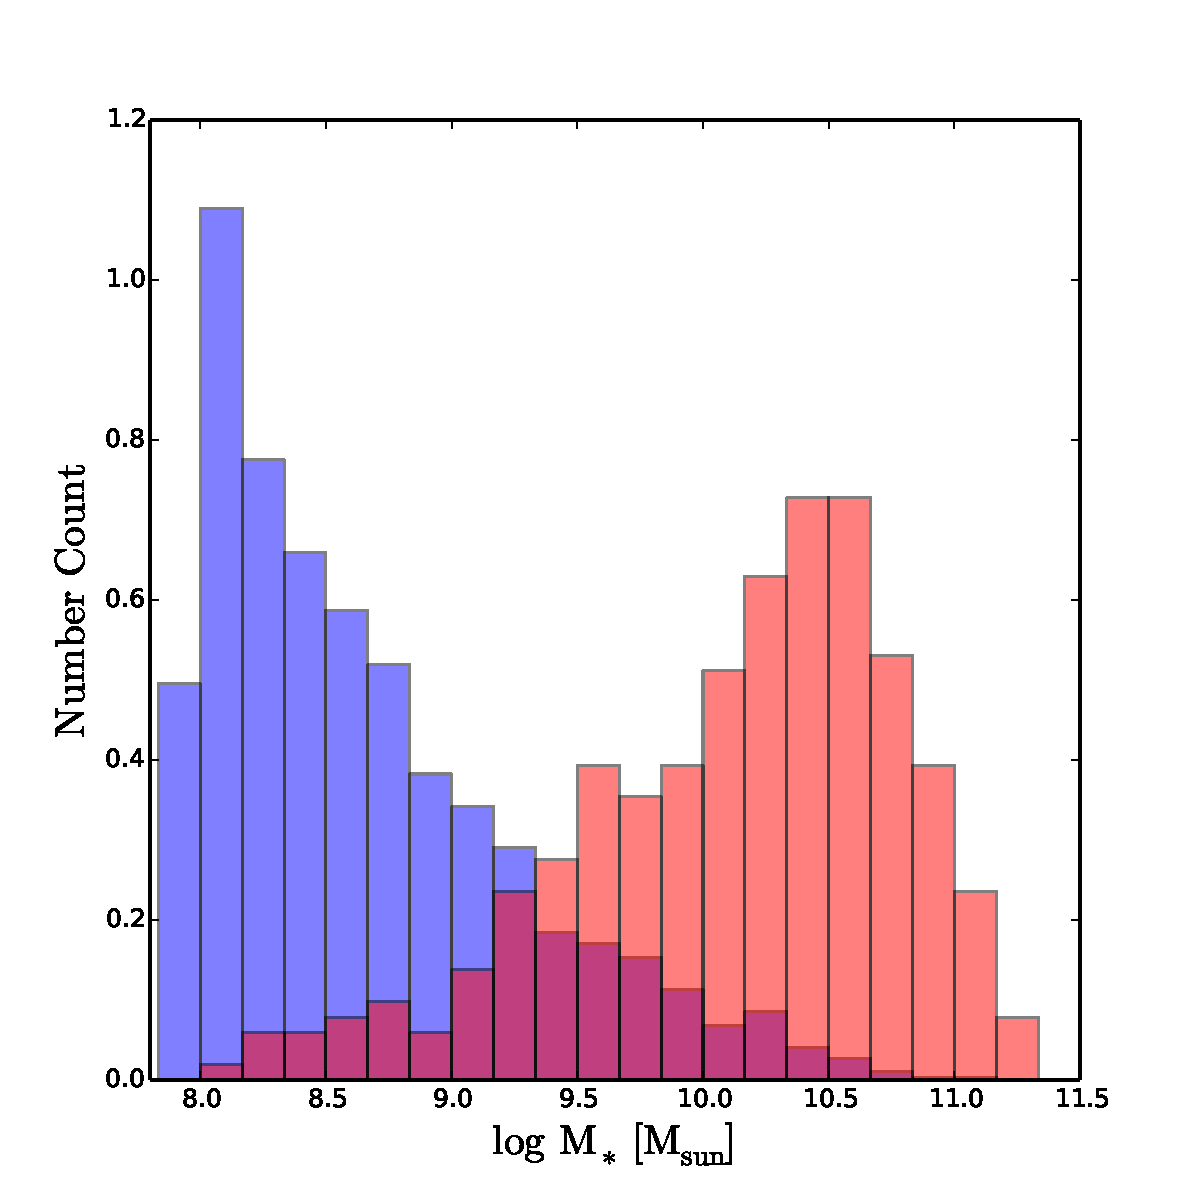
\includegraphics[width=\textwidth]{img/Hist.pdf}
								\caption{}
							\end{minipage}
							\begin{minipage}{0.32\textwidth}
								\centering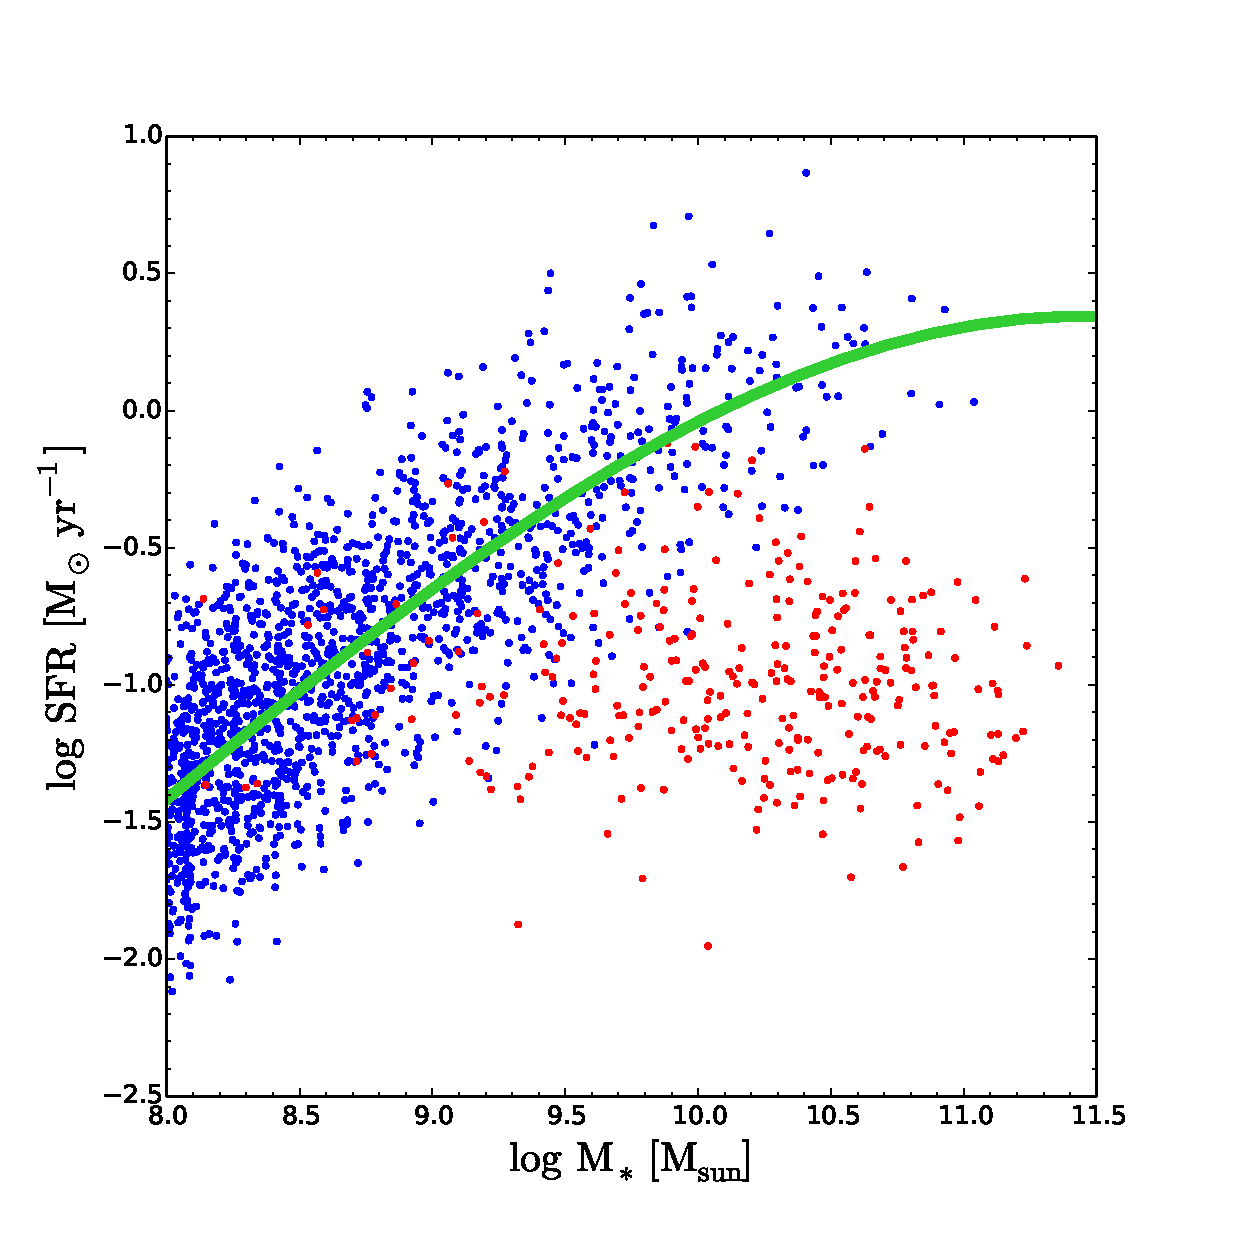
\includegraphics[width=\textwidth]{img/MSFR.eps}
								\caption{\cite{saintonge2016SFRMstar}}
							\end{minipage}
						\end{figure}

						\begin{figure}
							\begin{minipage}{0.32\textwidth}
								\centering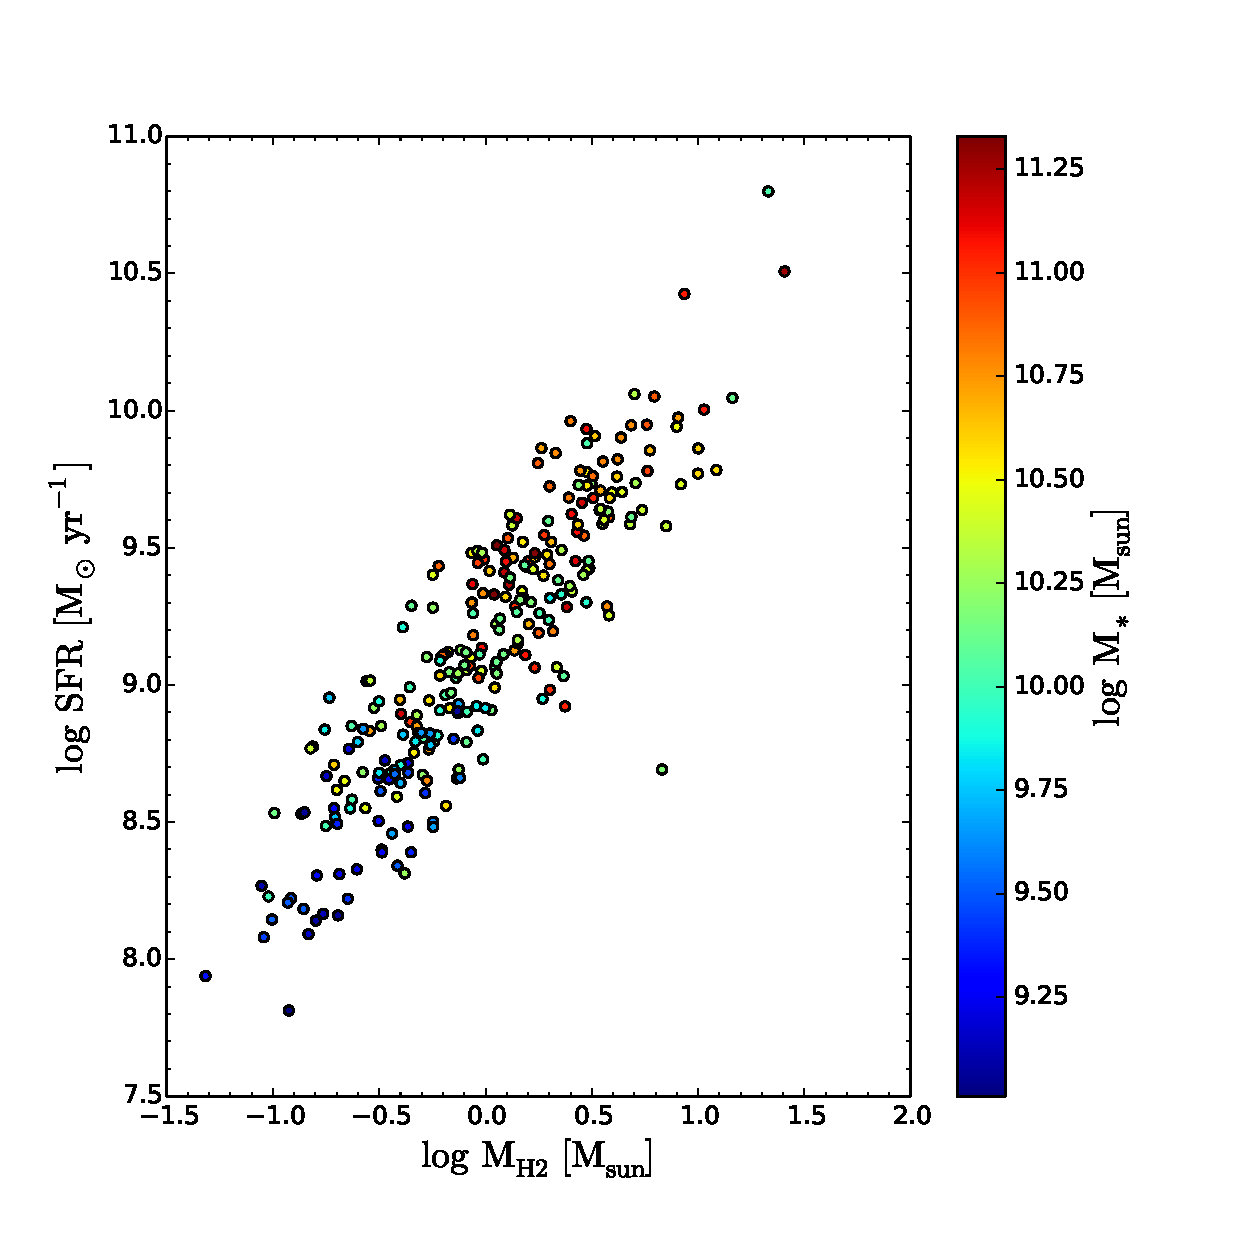
\includegraphics[width=\textwidth]{img/scalrelns.eps}
								\caption{}
							\end{minipage}
							\begin{minipage}{0.32\textwidth}
								\centering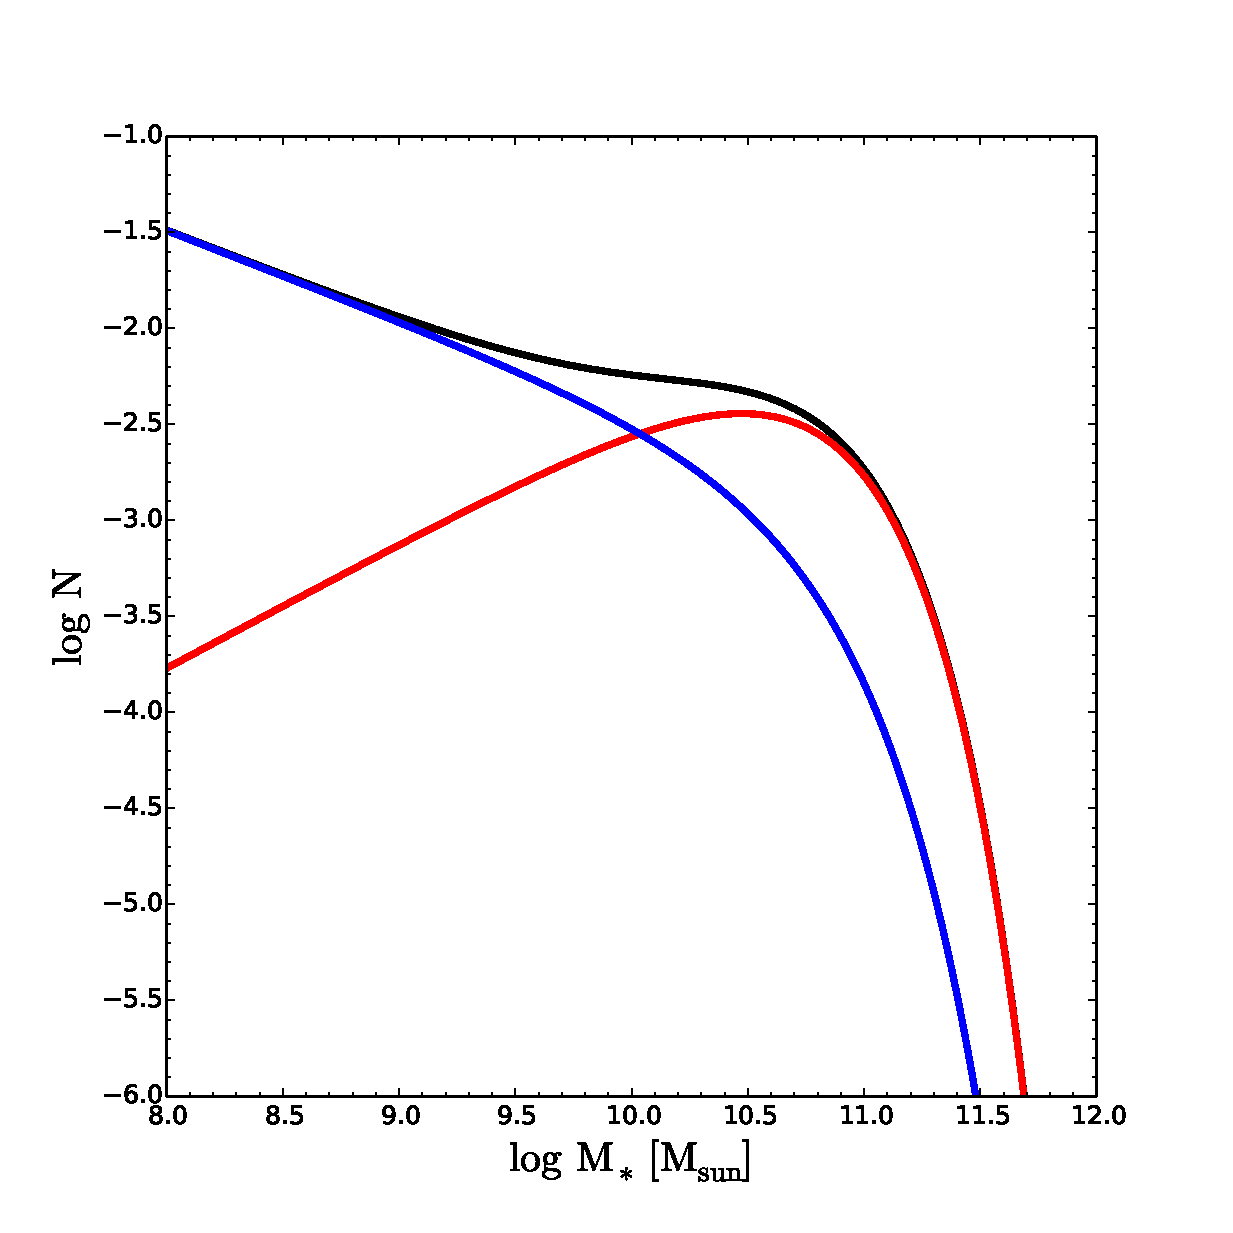
\includegraphics[width=\textwidth]{img/Baldry.eps}
								\caption{}
							\end{minipage}
							\begin{minipage}{0.32\textwidth}
								\centering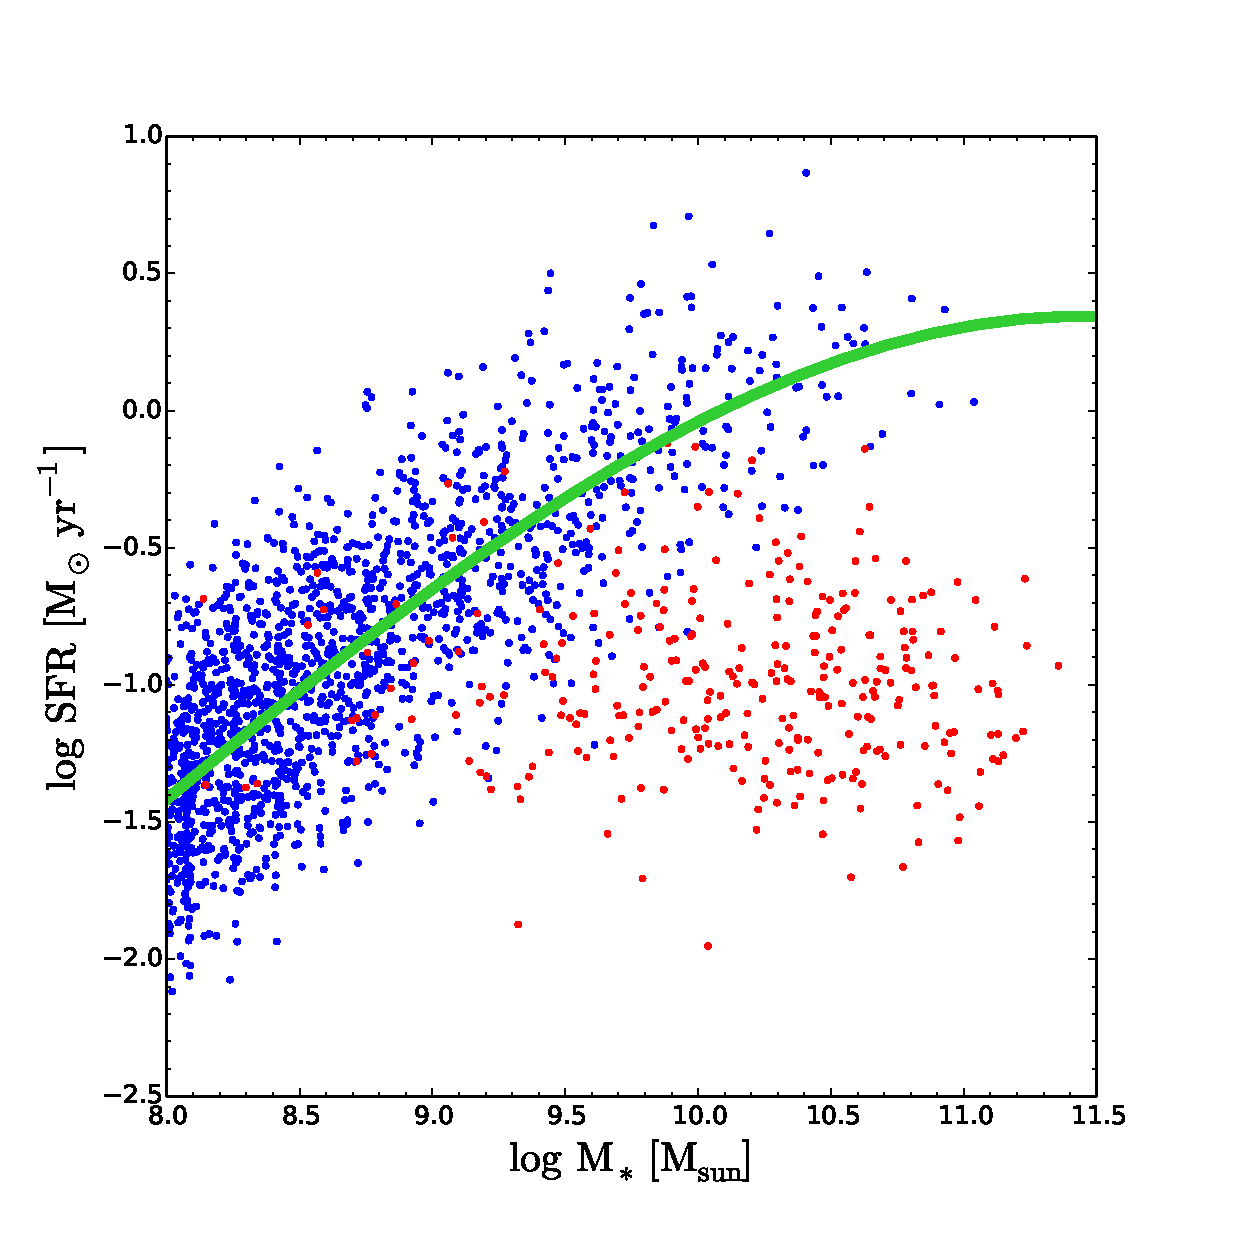
\includegraphics[width=\textwidth]{img/MSFR.eps}
								\caption{\cite{saintonge2016SFRMstar}}
							\end{minipage}
						\end{figure}
					\end{myblock}\vfill
%%%%%%%%%%%%%%%%%%%%%%%%%%%%%%%%%%%%%%%%%%%%%%%%%%%%%%%%%%%%%%%%%%%%%%%%%%%%%%%%
					\begin{myblock}{\LARGE References}
						\footnotesize
						\bibliographystyle{agsm}
						\bibliography{./bib}
					\end{myblock}\vfill
%%%%%%%%%%%%%%%%%%%%%%%%%%%%%%%%%%%%%%%%%%%%%%%%%%%%%%%%%%%%%%%%%%%%%%%%%%%%%%%%
		}\end{minipage}\end{beamercolorbox}
	\end{column}
\end{columns}
\end{frame}
\end{document}
